\documentclass{article}
\usepackage{amsfonts}
\usepackage{amsmath}
\usepackage{amsthm}
\usepackage{graphicx}
\usepackage[letterpaper, margin=1in]{geometry}
\usepackage{multicol}
\usepackage{graphpap}
%\usepackage{pdfpages}
\usepackage{enumerate}
\usepackage{tabularx}
\usepackage{framed}
\usepackage{lscape} 
\usepackage{tikz}
\usepackage{pgfplots}
\pgfplotsset{compat=1.15}

\usetikzlibrary{arrows, calc, patterns, positioning, shapes}
\newcommand{\degree}{$^{\circ}$}


\begin{document}
%\setlength{\columnsep}{1cm}
\begin{multicols}{2}
\begin{center}
	 \textbf{Complements of Kappa Mu Epsilon\\ (Math Club)}
\end{center} \normalsize
\textbf{Instructions:} The goal is to fill in the numbers \textbf{1} through \textbf{81} in the grid so that the numbers increase in the snake where the snake can only go up, down, left, or right.  For example, the blank box in the upper left corner must be a 51 because 51 has to be next to 50 and the 50 is stuck with only one blank box next adjacent.

\begin{center}
	\renewcommand{\arraystretch}{1.5} %\large
	\begin{tabular}{*{9}{|c}|} \hline
	49 & 48 & 47 & 46 & 45 & 4 & 5 & 6 & 7\\ \hline 
50 &  &  &  &  &  &  &  & 8\\ \cline{2-2}\hline 
81 &  &  &  &  &  &  &  & 13\\ \hline 
76 &  &  &  &  &  &  &  & 14\\ \hline 
75 &  &  &  &  &  &  &  & 19\\ \hline 
66 &  &  &  &  &  &  &  & 20\\ \hline 
65 &  &  &  &  &  &  &  & 21\\ \hline 
64 &  &  &  &  &  &  &  & 28\\ \hline 
63 & 62 & 61 & 60 & 33 & 32 & 31 & 30 & 29 \\ \hline 
	\end{tabular}
\end{center}
Like Math, Computer Science, Physics on Facebook : \texttt{https://tinyurl.com/MCSPFacebook}

%\vspace{.5in}

\begin{center}
	 \textbf{Complements of Kappa Mu Epsilon\\ (Math Club)}
\end{center} \normalsize
\textbf{Instructions:} The goal is to fill in the numbers \textbf{1} through \textbf{81} in the grid so that the numbers increase in the snake where the snake can only go up, down, left, or right.  For example, the blank box in the upper left corner must be a 51 because 51 has to be next to 50 and the 50 is stuck with only one blank box next adjacent.

\begin{center}
	\renewcommand{\arraystretch}{1.5} %\large
	\begin{tabular}{*{9}{|c}|} \hline
	49 & 48 & 47 & 46 & 45 & 4 & 5 & 6 & 7\\ \hline 
50 &  &  &  &  &  &  &  & 8\\ \cline{2-2}\hline 
81 &  &  &  &  &  &  &  & 13\\ \hline 
76 &  &  &  &  &  &  &  & 14\\ \hline 
75 &  &  &  &  &  &  &  & 19\\ \hline 
66 &  &  &  &  &  &  &  & 20\\ \hline 
65 &  &  &  &  &  &  &  & 21\\ \hline 
64 &  &  &  &  &  &  &  & 28\\ \hline 
63 & 62 & 61 & 60 & 33 & 32 & 31 & 30 & 29 \\ \hline 
	\end{tabular}
\end{center}
Like Math, Computer Science, Physics on Facebook : \texttt{https://tinyurl.com/MCSPFacebook}

\begin{center}
	 \textbf{Complements of Kappa Mu Epsilon\\ (Math Club)}
\end{center} \normalsize
\textbf{Instructions:} The goal is to fill in the numbers \textbf{1} through \textbf{81} in the grid so that the numbers increase in the snake where the snake can only go up, down, left, or right.  For example, the blank box in the upper left corner must be a 51 because 51 has to be next to 50 and the 50 is stuck with only one blank box next adjacent.

\begin{center}
	\renewcommand{\arraystretch}{1.5} %\large
	\begin{tabular}{*{9}{|c}|} \hline
	49 & 48 & 47 & 46 & 45 & 4 & 5 & 6 & 7\\ \hline 
50 &  &  &  &  &  &  &  & 8\\ \cline{2-2}\hline 
81 &  &  &  &  &  &  &  & 13\\ \hline 
76 &  &  &  &  &  &  &  & 14\\ \hline 
75 &  &  &  &  &  &  &  & 19\\ \hline 
66 &  &  &  &  &  &  &  & 20\\ \hline 
65 &  &  &  &  &  &  &  & 21\\ \hline 
64 &  &  &  &  &  &  &  & 28\\ \hline 
63 & 62 & 61 & 60 & 33 & 32 & 31 & 30 & 29 \\ \hline 
	\end{tabular}
\end{center}
Like Math, Computer Science, Physics on Facebook : \texttt{https://tinyurl.com/MCSPFacebook}

%\vspace{.5in}

\begin{center}
	 \textbf{Complements of Kappa Mu Epsilon\\ (Math Club)}
\end{center} \normalsize
\textbf{Instructions:} The goal is to fill in the numbers \textbf{1} through \textbf{81} in the grid so that the numbers increase in the snake where the snake can only go up, down, left, or right.  For example, the blank box in the upper left corner must be a 51 because 51 has to be next to 50 and the 50 is stuck with only one blank box next adjacent.

\begin{center}
	\renewcommand{\arraystretch}{1.5} %\large
	\begin{tabular}{*{9}{|c}|} \hline
	49 & 48 & 47 & 46 & 45 & 4 & 5 & 6 & 7\\ \hline 
50 &  &  &  &  &  &  &  & 8\\ \cline{2-2}\hline 
81 &  &  &  &  &  &  &  & 13\\ \hline 
76 &  &  &  &  &  &  &  & 14\\ \hline 
75 &  &  &  &  &  &  &  & 19\\ \hline 
66 &  &  &  &  &  &  &  & 20\\ \hline 
65 &  &  &  &  &  &  &  & 21\\ \hline 
64 &  &  &  &  &  &  &  & 28\\ \hline 
63 & 62 & 61 & 60 & 33 & 32 & 31 & 30 & 29 \\ \hline 
	\end{tabular}
\end{center}
Like Math, Computer Science, Physics on Facebook : \texttt{https://tinyurl.com/MCSPFacebook}

\end{multicols}
%Fold back on dotted lines and forward on dashed lines. \medskip

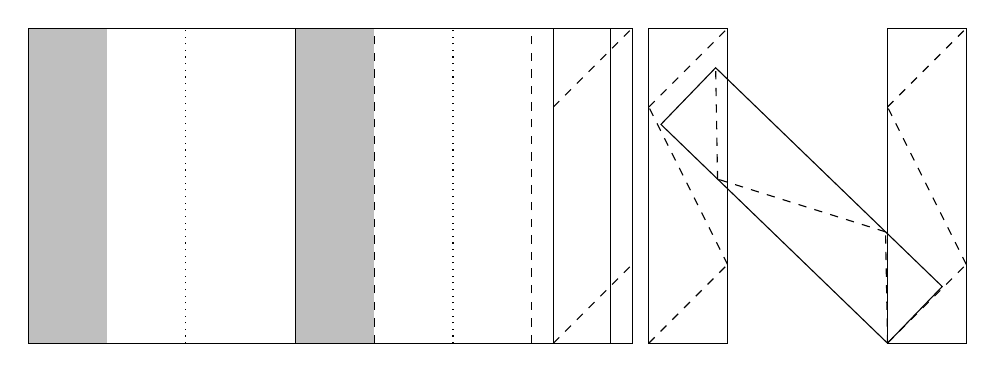
\begin{tikzpicture}
	\begin{scope}
	\draw[fill=lightgray, draw=none] (0,0) --(1,0) -- (1,4) -- (0,4) -- cycle;
		\draw (0,0) -- (4,0) -- (4,4) -- (0,4) -- cycle;
	\draw[dotted] (2,0) -- (2,4);
	\end{scope}
	
	\begin{scope}[xshift=.28\textwidth]
	\draw[fill=lightgray, draw=none] (0,0) --(1,0) -- (1,4) -- (0,4) -- cycle;
		\draw (0,0) -- (4,0) -- (4,4) -- (0,4) -- cycle;
	\draw[dotted] (2,0) -- (2,4);
\draw[dashed] (1,0) -- (1,4);
	\draw[dashed] (3,0) -- (3,4);
		
	\end{scope}
	
	\begin{scope}[xshift=.55\textwidth]
		\draw[] (0,0) --(1,0) -- (1,4) -- (0,4) -- cycle;
		\draw[dashed] (0,0) -- (1,1);
		\draw[dashed] (0,3) -- (1,4);
	\end{scope}

\begin{scope}[xshift = .65\textwidth]
		\draw[] (0,0) --(1,0) -- (1,4) -- (0,4) -- cycle;
		\draw[dashed] (0,0) -- (1,1);
		\draw[dashed] (0,3) -- (1,4);
		\draw[dashed] (1,1) -- (0,3);
	\end{scope}
	
	\begin{scope}[xshift=.9\textwidth]
			\begin{scope}
		\draw[] (0,0) --(1,0) -- (1,4) -- (0,4) -- cycle;
		\draw[dashed] (0,0) -- (1,1);
		\draw[dashed] (0,3) -- (1,4);
		\draw[dashed] (1,1) -- (0,3);
	\end{scope}
	
	\begin{scope}[rotate=46]
		\draw[] (0,0) --(1,0) -- (1,4) -- (0,4) -- cycle;
		\draw[dashed] (0,0) -- (1,1);
		\draw[dashed] (0,3) -- (1,4);
		\draw[dashed] (1,1) -- (0,3);
	\end{scope}

	\end{scope}
\end{tikzpicture}

\vfill

Fold back on dotted lines and forward on dashed lines. \medskip

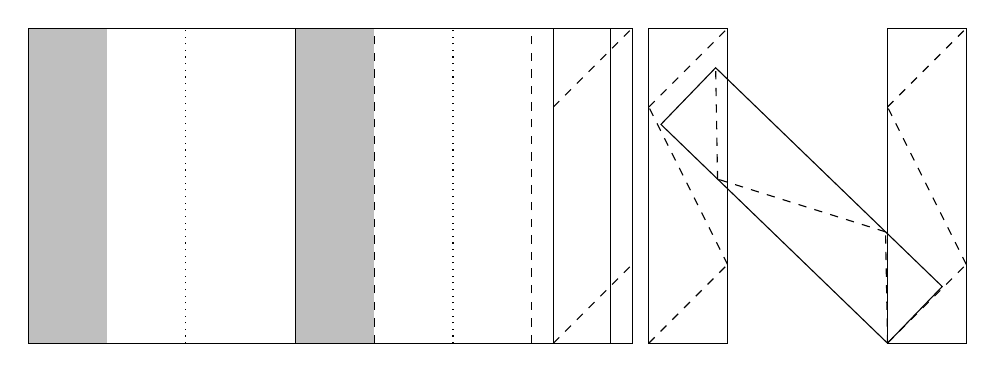
\begin{tikzpicture}
	\begin{scope}
	\draw[fill=lightgray, draw=none] (0,0) --(1,0) -- (1,4) -- (0,4) -- cycle;
		\draw (0,0) -- (4,0) -- (4,4) -- (0,4) -- cycle;
	\draw[dotted] (2,0) -- (2,4);
	\end{scope}
	
	\begin{scope}[xshift=.28\textwidth]
	\draw[fill=lightgray, draw=none] (0,0) --(1,0) -- (1,4) -- (0,4) -- cycle;
		\draw (0,0) -- (4,0) -- (4,4) -- (0,4) -- cycle;
	\draw[dotted] (2,0) -- (2,4);
\draw[dashed] (1,0) -- (1,4);
	\draw[dashed] (3,0) -- (3,4);
		
	\end{scope}
	
	\begin{scope}[xshift=.55\textwidth]
		\draw[] (0,0) --(1,0) -- (1,4) -- (0,4) -- cycle;
		\draw[dashed] (0,0) -- (1,1);
		\draw[dashed] (0,3) -- (1,4);
	\end{scope}

\begin{scope}[xshift = .65\textwidth]
		\draw[] (0,0) --(1,0) -- (1,4) -- (0,4) -- cycle;
		\draw[dashed] (0,0) -- (1,1);
		\draw[dashed] (0,3) -- (1,4);
		\draw[dashed] (1,1) -- (0,3);
	\end{scope}
	
	\begin{scope}[xshift=.9\textwidth]
			\begin{scope}
		\draw[] (0,0) --(1,0) -- (1,4) -- (0,4) -- cycle;
		\draw[dashed] (0,0) -- (1,1);
		\draw[dashed] (0,3) -- (1,4);
		\draw[dashed] (1,1) -- (0,3);
	\end{scope}
	
	\begin{scope}[rotate=46]
		\draw[] (0,0) --(1,0) -- (1,4) -- (0,4) -- cycle;
		\draw[dashed] (0,0) -- (1,1);
		\draw[dashed] (0,3) -- (1,4);
		\draw[dashed] (1,1) -- (0,3);
	\end{scope}

	\end{scope}
\end{tikzpicture}



\vfill

Fold back on dotted lines and forward on dashed lines. \medskip

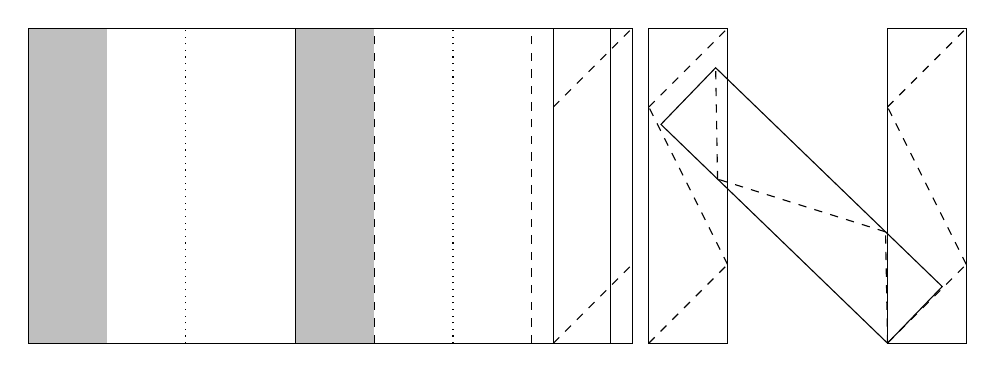
\begin{tikzpicture}
	\begin{scope}
	\draw[fill=lightgray, draw=none] (0,0) --(1,0) -- (1,4) -- (0,4) -- cycle;
		\draw (0,0) -- (4,0) -- (4,4) -- (0,4) -- cycle;
	\draw[dotted] (2,0) -- (2,4);
	\end{scope}
	
	\begin{scope}[xshift=.28\textwidth]
	\draw[fill=lightgray, draw=none] (0,0) --(1,0) -- (1,4) -- (0,4) -- cycle;
		\draw (0,0) -- (4,0) -- (4,4) -- (0,4) -- cycle;
	\draw[dotted] (2,0) -- (2,4);
\draw[dashed] (1,0) -- (1,4);
	\draw[dashed] (3,0) -- (3,4);
		
	\end{scope}
	
	\begin{scope}[xshift=.55\textwidth]
		\draw[] (0,0) --(1,0) -- (1,4) -- (0,4) -- cycle;
		\draw[dashed] (0,0) -- (1,1);
		\draw[dashed] (0,3) -- (1,4);
	\end{scope}

\begin{scope}[xshift = .65\textwidth]
		\draw[] (0,0) --(1,0) -- (1,4) -- (0,4) -- cycle;
		\draw[dashed] (0,0) -- (1,1);
		\draw[dashed] (0,3) -- (1,4);
		\draw[dashed] (1,1) -- (0,3);
	\end{scope}
	
	\begin{scope}[xshift=.9\textwidth]
		\draw[] (0,0) --(1,0) -- (1,4) -- (0,4) -- cycle;
		\draw[dashed] (0,0) -- (1,1);
		\draw[dashed] (0,3) -- (1,4);
		\draw[dashed] (1,1) -- (0,3);
	
		\begin{scope}[rotate=46]
		\draw[] (0,0) --(1,0) -- (1,4) -- (0,4) -- cycle;
		\draw[dashed] (0,0) -- (1,1);
		\draw[dashed] (0,3) -- (1,4);
		\draw[dashed] (1,1) -- (0,3);
	\end{scope}

	\end{scope}
\end{tikzpicture}


%\begin{landscape}

\begin{tabular}{p{2in}p{2in}p{2in}p{2in}}
\centering
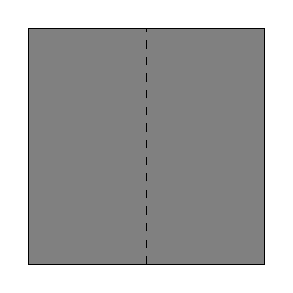
\begin{tikzpicture}[scale=.75]
	\draw[fill=gray] (0,0) rectangle (4,4);
	\draw[dashed] (2,0) -- (2,4);
\end{tikzpicture}

Fold paper in half 
	& 
{\centering
	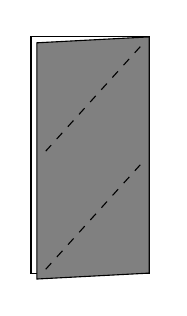
\begin{tikzpicture}[scale=.75]
		\draw (0,0) rectangle (2,4);
		\draw[fill=gray] (.1,-.1) node (A) {} -- (2,0) -- (2,4) node[pos=.5] (B) {} node (C) {}-- (.1,3.9)  -- cycle node[pos=.5] (D) {};
		\draw[dashed] (A) -- (B);
		\draw[dashed] (C) -- (D);
	\end{tikzpicture}}
	
Bring one corner to opposite edge to form a triangle and repeat with opposite corner	
	& 
\centering	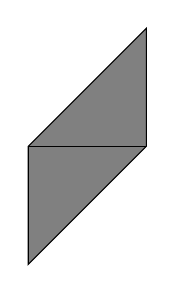
\begin{tikzpicture}[scale=.75]
		\draw[fill=gray] (0,0) -- (2,2) -- (2,4) -- (0,2) --cycle;
		\draw (0,2) -- (2,2);
	\end{tikzpicture}
	
	You should see a parallelogram
	& 
	\centering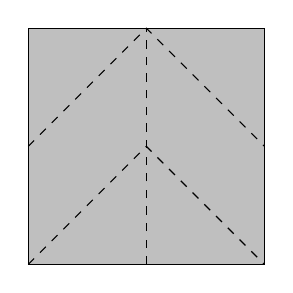
\begin{tikzpicture}[scale=.75]
	\draw[fill=lightgray] (0,0) rectangle (4,4);
	\draw[dashed] (2,0) -- (2,4);
		\draw[dashed] (0,0) -- (2,2) -- (4,0);
		\draw[dashed] (0,2) -- (2,4) -- (4,2);
\end{tikzpicture}

Open the paper
	\end{tabular}
	
	\begin{tabular}{p{2in}p{2in}p{2in}p{2in}}

	
	{\centering 
	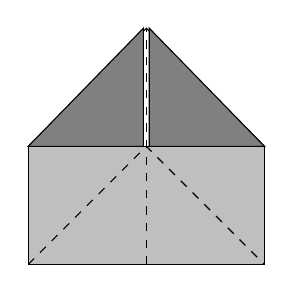
\begin{tikzpicture}[scale=.75]
	\begin{scope}
			\draw[fill=lightgray] (0,0) rectangle (4,2);
	\draw (0,2) -- (2,4) -- (4,2);
	\draw[dashed] (2,0) -- (2,4);
		\draw[dashed] (0,0) -- (2,2) -- (4,0);
		\draw[fill=gray] (0,2) -- (1.95,4) -- (1.95,2) -- cycle;
		\draw[fill=gray] (4,2) -- (2.05,4) -- (2.05,2) -- cycle;
	\end{scope}
	\begin{scope}[xshift=2in]
		(0,0) to[bend right] (2,0);
	\end{scope}
	\end{tikzpicture}
	
	Fold top two corners to the centering and flip the paper over.}
	&
	{\centering 
	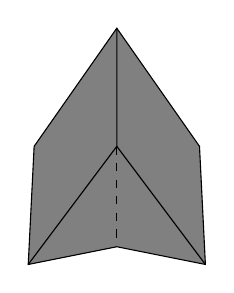
\begin{tikzpicture}[scale=.75]
		\draw[fill=gray] (0,0) -- (.1,2) -- (1.5,4) -- (2.9,2) -- (3,0) -- (1.5,.3) -- cycle;
		\draw (0,0) -- (1.5,2) -- (1.5,4);
		\draw (3,0) -- (1.5,2);
		\draw[dashed] (1.5,2) -- (1.5,.3);
	\end{tikzpicture}}
	
	Push the large triangular region inside
	&
	{\centering 
	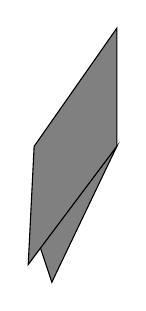
\begin{tikzpicture}[scale=.75]
		\draw[fill=gray] (1.5,2) -- (.4,-.3) -- (.2,.3) -- cycle;
		\draw[fill=gray] (0,0) -- (.1,2) -- (1.5,4) -- (1.5,2) -- cycle;
	\end{tikzpicture}}
	
	Flatten the parallelogram to complete the module.  Make seven more modules.
	&
	{\centering
	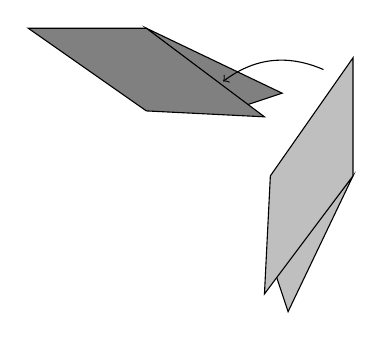
\begin{tikzpicture}[scale=.75]
		\begin{scope}[rotate=90]
					\draw[fill=gray] (1.5,2) -- (.4,-.3) -- (.2,.3) -- cycle;
		\draw[fill=gray] (0,0) -- (.1,2) -- (1.5,4) -- (1.5,2) -- cycle;
		\end{scope}
		\begin{scope}[xshift=0cm, yshift=-3cm]
					\draw[fill=lightgray] (1.5,2) -- (.4,-.3) -- (.2,.3) -- cycle;
		\draw[fill=lightgray] (0,0) -- (.1,2) -- (1.5,4) -- (1.5,2) -- cycle;
		\draw[->] (1,3.8) to[bend right] (-.7,3.6);
		\end{scope}
	\end{tikzpicture}}
	
	Insesrt one piece into another so that the folded edge of each module is on the outside
	\end{tabular}
	
	\begin{tabular}{p{2in}p{2in}p{2in}p{2in}}

	\centering
		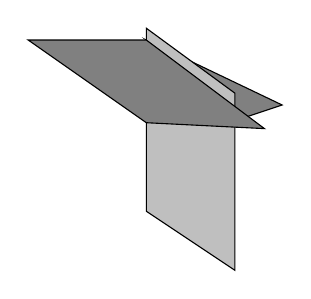
\begin{tikzpicture}[scale=.75]
		\begin{scope}[rotate=90]
					\draw[fill=gray] (1.5,2) -- (.4,-.3) -- (.2,.3) -- cycle;
% 		\draw[fill=gray] (0,0) -- (.1,2) -- (1.5,4) -- (1.5,2) -- cycle;
		\end{scope}
		\begin{scope}[xshift=-2cm, yshift=-1.4cm]
			\draw[fill=lightgray] (0,0) -- (0,3.1) -- (1.5,2) -- (1.5,-1) -- cycle;
		\end{scope}
		\begin{scope}[rotate=90]
				% 	\draw[fill=gray] (1.5,2) -- (.4,-.3) -- (.2,.3) -- cycle;
		\draw[fill=gray] (0,0) -- (.1,2) -- (1.5,4) -- (1.5,2) -- cycle;
		\end{scope}
		
	\end{tikzpicture}
	Be sure to tuck the inside piece as far into the fold as possible
	&
	\centering
		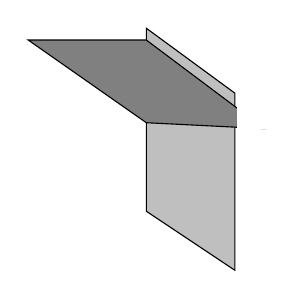
\begin{tikzpicture}[scale=.75]
		\begin{scope}[xshift=-2cm, yshift=-1.4cm]
			\draw[fill=lightgray] (0,0) -- (0,3.1) -- (1.5,2) -- (1.5,-1) -- cycle;
		\end{scope}
		\begin{scope}[rotate=90]
				% 	\draw[fill=gray] (1.5,2) -- (.4,-.3) -- (.2,.3) -- cycle;
		\draw[fill=gray] (0,0) -- (.1,2) -- (1.5,4) -- (1.5,2) -- cycle;
		\end{scope}
		\begin{scope}[yshift=0cm, xshift=-.45cm]
		    \draw[white, fill=white] (0,0) rectangle (.5,.5);
		\end{scope}
		
	\end{tikzpicture}
	Tuck the corners of the outside module into the grove of the inside module as snuggly as possible
	&
	{\centering
	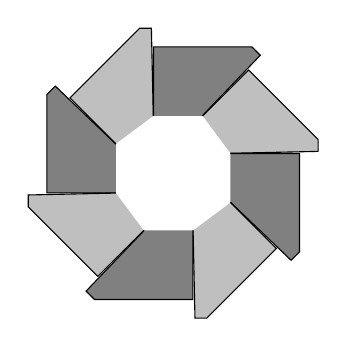
\begin{tikzpicture}[scale=.5]
	    \draw[white] (-1,0) node (A) {} -- ++(90:1) node (B) {} -- ++(45:1) node (C) {}-- ++(0:1) node (D) {}-- ++(-45:1) node (E) {}-- ++(-90:1) node (F) {}-- ++(-135:1) node (G) {}-- ++(-180:1) node (H) {}-- ++(-225:1) -- cycle ;
	    \draw[fill=gray] (A) -- ++(180:2) -- ++ (90:2.5)-- ++ (45:.3) -- (B) -- cycle ;
	    \draw[fill=lightgray] (B) -- ++(135:2) -- ++ (45:2.5)-- ++ (0:.3) -- (C) -- cycle ;
	    \draw[fill=gray] (C) -- ++(90:2) -- ++ (0:2.5)-- ++ (-45:.3) -- (D) -- cycle ;
	    \draw[fill=lightgray] (D) -- ++(45:2) -- ++ (-45:2.5)-- ++ (-90:.3) -- (E) -- cycle ;
	    \draw[fill=gray] (E) -- ++(0:2) -- ++ (-90:2.5)-- ++ (-135:.3) -- (F) -- cycle ;
	    \draw[fill=lightgray] (F) -- ++(-45:2) -- ++ (-135:2.5)-- ++ (-180:.3) -- (G) -- cycle ;
	    \draw[fill=gray] (G) -- ++(-90:2) -- ++ (-180:2.5)-- ++ (-225:.3) -- (H) -- cycle ;
	    \draw[fill=lightgray] (H) -- ++(-135:2) -- ++ (-225:2.5)-- ++ (-270:.3) -- (A) -- cycle ;
	\end{tikzpicture}}
	
	Continue to add modules around the octagon.  Tuck the corners of the last module on either side of the parallelogram inside the first module.
	&
	{\centering
	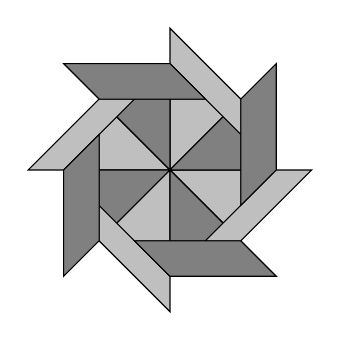
\begin{tikzpicture}[scale=.9]
	    \foreach \t in {90,0,-90,-180} {\draw[fill=lightgray] (0,0) -- ++(\t:1) -- ++ ({\t-90}:1) -- cycle; }
	    \foreach \t in {90,0,-90,-180} {\draw[fill=gray] (0,0) -- ++(\t:1) -- ++ ({\t+90}:1) -- cycle; }
	   	   \draw[fill=lightgray] (0,1.5) -- ++(0,.5) -- ++(1,-1) -- ++(0, -.5) -- cycle;
	   	   \draw[fill=lightgray] (1.5,0) -- ++(.5,0) -- ++(-1,-1) -- ++(-.5, 0) -- cycle;
	   	   \draw[fill=lightgray] (0,-1.5) -- ++(0,-.5) -- ++(-1,1) -- ++(0, .5) -- cycle;
	   	   \draw[fill=lightgray] (-1.5,0) -- ++(-.5,0) -- ++(1,1) -- ++(.5, 0) -- cycle;
	   	     \draw[fill=gray] (0,1.5) -- ++(.5,-.5) -- ++(-1.5,0) -- ++(-.5, .5) -- cycle;
	   	   \draw[fill=gray] (1.5,0) -- ++(-.5,-.5) -- ++(0,1.5) -- ++(.5, .5) -- cycle;
	   	   \draw[fill=gray] (0,-1.5) -- ++(-.5,.5) -- ++(1.5,0) -- ++(.5, -.5) -- cycle;
	   	   \draw[fill=gray] (-1.5,0) -- ++(.5,.5) -- ++(0,-1.5) -- ++(-.5, -.5) -- cycle;
	\end{tikzpicture}}
	
	Push gently to transform into a pinwheel.  If necessary, sharpen the creases and slide it in and out a few times.
\end{tabular} 

\end{landscape}
%	\begin{enumerate}
		\item How many different ways are there to place the dominoes in a $2\times n$ hallway?
		
		$n=1$
		\begin{tikzpicture}[scale=2]
			\draw (0 ,0 ) -- (0 , 2  ) -- (1 , 2  ) -- (1 ,0 )--cycle;
		\end{tikzpicture} \hfill
		$n=2$
		\begin{tikzpicture}[scale=2]
			\draw (0 ,0 ) -- (0 , 2  ) -- (2 , 2  ) -- (2 ,0 )--cycle;
		\end{tikzpicture}
		\hfill
		$n=3$
		\begin{tikzpicture}[scale=2]
			\draw (0 ,0 ) -- (0 , 2  ) -- (3 , 2  ) -- (3 ,0 )--cycle;
		\end{tikzpicture}

		$n=4$
		\begin{tikzpicture}[scale=2]
			\draw (0 ,0 ) -- (0 , 2  ) -- (4 , 2  ) -- (4 ,0 )--cycle;
		\end{tikzpicture}

		$n=5$
		\begin{tikzpicture}[scale=2]
			\draw (0 ,0 ) -- (0 , 2  ) -- (5 , 2  ) -- (5 ,0 )--cycle;
		\end{tikzpicture}
		
			$n=6$
		\begin{tikzpicture}[scale=2]
			\draw (0 ,0 ) -- (0 , 2  ) -- (6 , 2  ) -- (6 ,0 )--cycle;
		\end{tikzpicture}
		\item What would be a formula for a general $n$?  Explain why the pattern and formula work.
		
\clearpage
		\item There are three ways to dissect a $3\times 2$ rectangle into
dominos. How many ways are there to dissect a $3\times 4$ rectangle into dominos?

\begin{tikzpicture}[scale=2]
			\draw (0 ,0 ) -- (0 , 3  ) -- (4 , 3  ) -- (4 ,0 )--cycle;
\end{tikzpicture}
		
	\item It is not possible to dissect a $3\times1$ rectangle into dominos. Likewise it is not possible to
dissect $3\times3 3\times5, 3\times7$,… rectangles into dominos. Suppose we remove a single $1\times1$
square from the lower left corner of these rectangles (we’ll call these shapes the $3\times1-
1, 3\times3-1, 3\times5-1$,…). These shapes can be dissected into dominos. Below we show, for
example, how to dissect the $3\times1-1$ shape, $3\times3-1$ shape, and $3\times5-1$ shape into dominos.
How many ways are there to dissect a $3\times3-1$ rectangle into dominos? A $3\times5-1$
rectangle into dominos?

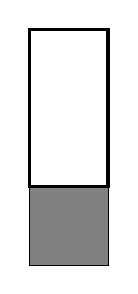
\begin{tikzpicture}[scale=1]
			\draw (0 ,0 ) -- (1 , 0) -- (1 , 3) -- (0 , 3)--cycle;
			\draw[fill=gray] (0 ,0 ) -- (0 , 1) -- (1 , 1) -- (1 ,0 )--cycle;
			\draw[very thick] (0, 1) -- (1 , 1) -- (1 , 3) -- (0 , 3)--cycle;
\end{tikzpicture} \hfill
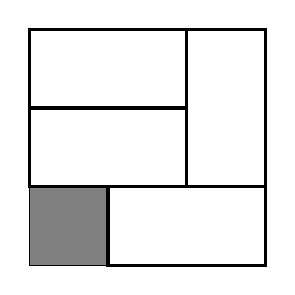
\begin{tikzpicture}[scale=1]
			\draw (0 ,0 ) -- (3 , 0) -- (3 , 3) -- (0 , 3)--cycle;
			\draw[fill=gray] (0 ,0 ) -- (0 , 1) -- (1 , 1) -- (1 ,0 )--cycle;
			\draw[very thick] (1, 0) -- (3 , 0) -- (3 , 1) -- (1 , 1)--cycle;
			\draw[very thick] (0, 1) -- (2 , 1) -- (2 , 2) -- (0 , 2)--cycle;
			\draw[very thick] (0, 2) -- (2 , 2) -- (2 , 3) -- (0 , 3)--cycle;
			\draw[very thick] (2, 1) -- (3 , 1) -- (3 , 3) -- (2 , 3)--cycle;
\end{tikzpicture}\hfill
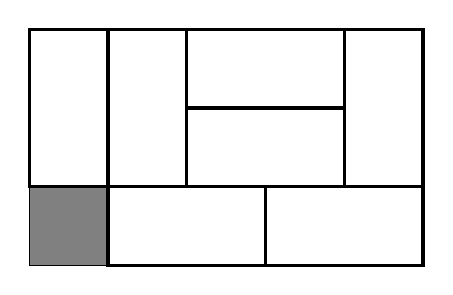
\begin{tikzpicture}[scale=1]
			\draw (0 ,0 ) -- (5 , 0) -- (5 , 3) -- (0 , 3)--cycle;
			\draw[fill=gray] (0 ,0 ) -- (0 , 1) -- (1 , 1) -- (1 ,0 )--cycle;
			\draw[very thick] (1, 0) -- (3 , 0) -- (3 , 1) -- (1 , 1)--cycle;
			\draw[very thick] (3, 0) -- (5 , 0) -- (5 , 1) -- (3 , 1)--cycle;
			\draw[very thick] (0, 1) -- (1 , 1) -- (1 , 3) -- (0 , 3)--cycle;
			\draw[very thick] (1, 1) -- (2 , 1) -- (2 , 3) -- (1 , 3)--cycle;
			\draw[very thick] (2, 1) -- (4 , 1) -- (4 , 2) -- (2 , 2)--cycle;
			\draw[very thick] (2, 2) -- (4 , 2) -- (4 , 3) -- (2 , 3)--cycle;
			\draw[very thick] (4, 1) -- (4 , 3) -- (5 , 3) -- (5 , 1)--cycle;
\end{tikzpicture}

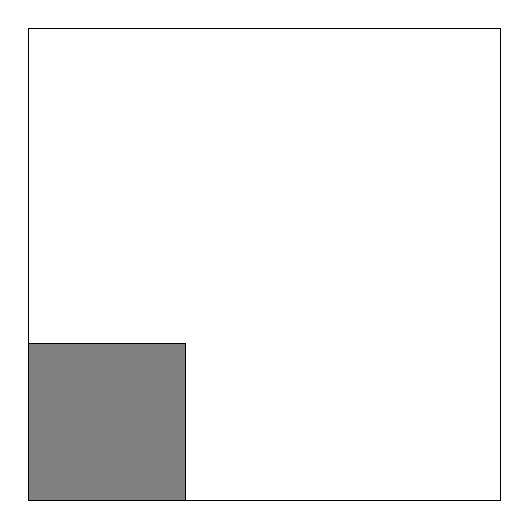
\begin{tikzpicture}[scale=2]
			\draw (0 ,0 ) -- (3 , 0) -- (3 , 3) -- (0 , 3)--cycle;
			\draw[fill=gray] (0 ,0 ) -- (0 , 1) -- (1 , 1) -- (1 ,0 )--cycle;
\end{tikzpicture}
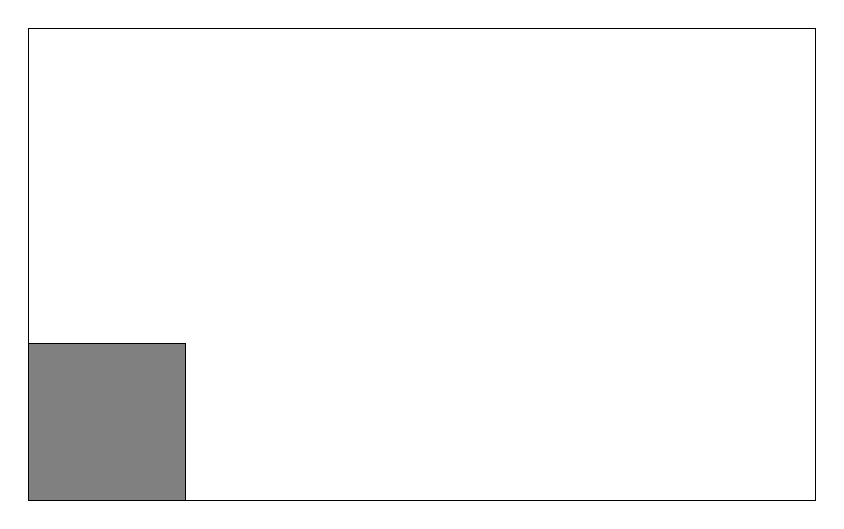
\begin{tikzpicture}[scale=2]
				\draw (0 ,0 ) -- (5 , 0) -- (5 , 3) -- (0 , 3)--cycle;
			\draw[fill=gray] (0 ,0 ) -- (0 , 1) -- (1 , 1) -- (1 ,0 )--cycle;
\end{tikzpicture}
	\end{enumerate}
	\clearpage
	

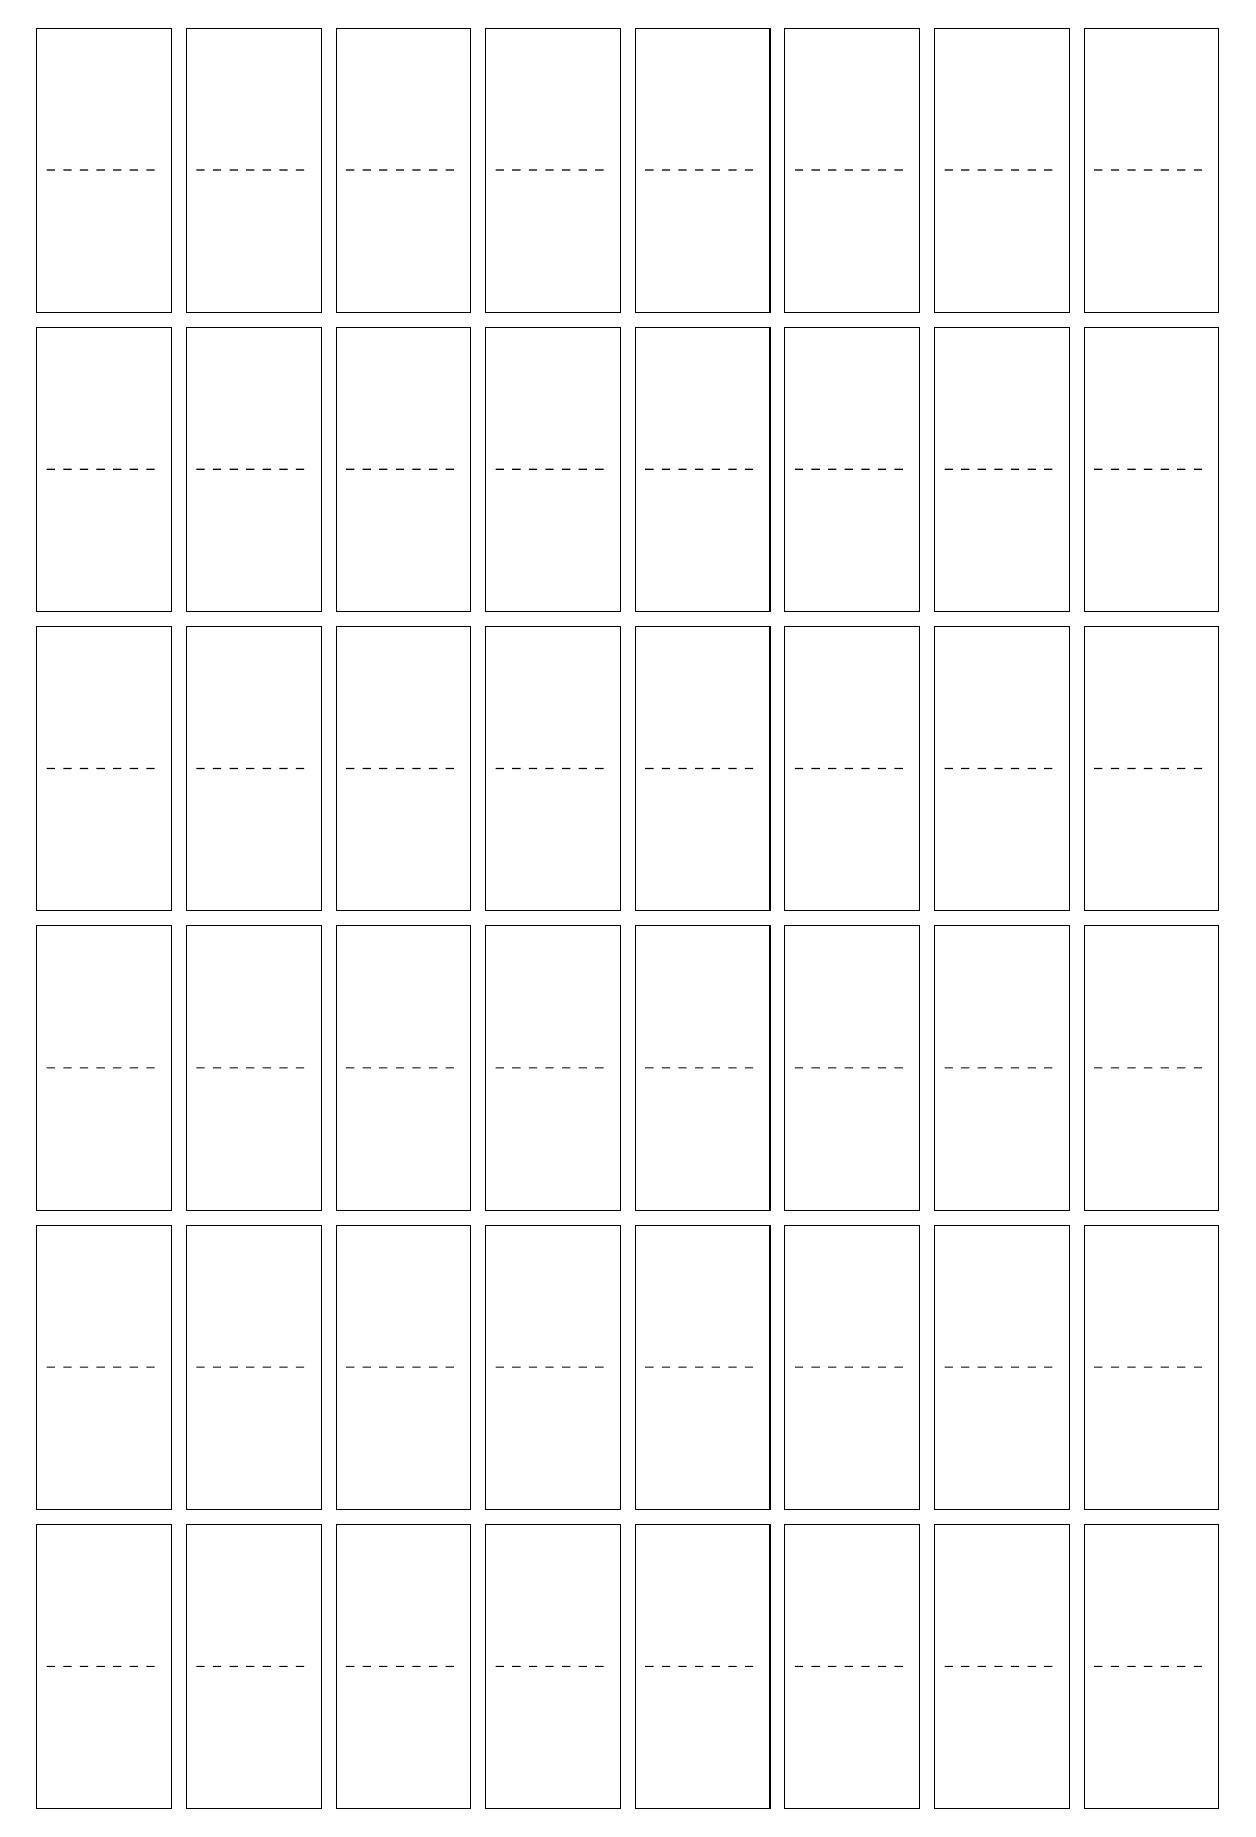
\begin{tikzpicture}[scale=1.9]
\foreach \y in {0,2,...,10}
\foreach \x in {0,1,...,7}{
			\draw (\x ,\y ) -- (\x , 2+\y  -.1) node[pos=.5] (1) {} -- (\x +1  -.1, 2+\y   -.1) -- (\x +1  -.1, \y )  node[pos=.5] (2) {}--cycle;
			\draw[dashed] (1)--(2);}
		
	\end{tikzpicture}
	\clearpage

%{\Large Ultimate Tic-Tac-Toe\footnote{From \underline{Math with Bad Drawings} by Ben Orlin}}

\begin{enumerate}
	\item Each turn you mark a square on a mini-board.
	\item You don’t get to pick which of the nine boards to play on. That’s determined by your opponent’s previous move. Whichever square he picks, that’s the board you must play in next.  The exception to this rule is if the board you are sent to has already been won, you can go to any mini-board you wish.
	\item When you get three in a row on a mini-board, you win that board.
	\item When you get three mini-boards in a row, you win the game.
\end{enumerate}
\vspace{1cm}
\centering

\begin{tikzpicture}[scale=.5]
		\draw (-5,-15) -- ++(90:30);
		\draw (5,-15) -- ++(90:30);
		\draw (-15,-5) -- ++(0:30);
		\draw (-15,5) -- ++(0:30);
\foreach \x in {-4,0,4}
\foreach \y in {-4,0,4}
	{\begin{scope}[xshift=\x in, yshift = \y in]
		\draw (-1,-3) -- ++(90:6);
		\draw (1,-3) -- ++(90:6);
		\draw (-3,-1) -- ++(0:6);
		\draw (-3,1) -- ++(0:6);
	\end{scope}}

\end{tikzpicture}
%\newcommand{\cools}{
\begin{tikzpicture}[scale = 0.08]
	\draw[] (1, -3)--(1, -2)--(0,-1) --(0,0) -- (1, 1) -- (2, 0) -- (2,-1) -- (1.5, -1.5);
	\draw[] (0.5, -1.5) -- (0, -2)-- (0, -3) -- (1, -4) -- (2, -3) -- (2, -2) -- (1, -1) -- (1,0);
\end{tikzpicture}}
\large
\textbf{Play \cools
}

\section*{Cool S Game}
Start with a grid with alternating
vertical lines drawn in. Take it in
turns to add a diagonal line (full or
partial). If you create a \cools \, 
shape in the grid, write your initial
in it.

The winner is the player with the
most \cools 's drawn in the grid
when no more moves are
possible. \medskip

\begin{center}
\begin{tikzpicture}

\foreach \y in {0,...,8}{
	 \foreach \x in {0,...,15}{
		\draw (0.5*\x,\y) -- (0.5*\x,\y + 0.5);
		}
	}
	
	\foreach \x in {0,...,15}{
		\fill (0.5*\x,9) circle[radius=0.5pt];
		\fill (0.5*\x,-0.5) circle[radius=0.5pt];
		}

\end{tikzpicture}\vfill

\begin{tikzpicture}

\foreach \y in {0,...,8}{
	 \foreach \x in {0,...,15}{
		\draw (0.5*\x,\y) -- (0.5*\x,\y + 0.5);
		}
	}
	
	\foreach \x in {0,...,15}{
		\fill (0.5*\x,9) circle[radius=0.5pt];
		\fill (0.5*\x,-0.5) circle[radius=0.5pt];
		}

\end{tikzpicture}\medskip \\


	\begin{tikzpicture}
	
\foreach \y in {0,...,20}{
	 \foreach \x in {0,...,30}{
		\draw [] (0.5*\x,\y) -- (0.5*\x,\y + 0.5);
		}
	}
	
	\foreach \x in {0,...,30}{
		\fill (0.5*\x,21) circle[radius=0.5pt];
		\fill (0.5*\x,-0.5) circle[radius=0.5pt];
		}

\end{tikzpicture}
\end{center}

\section*{Paper Boxing}
\vfill
\begin{center}
	\begin{tikzpicture}[scale=2]
		\draw[step=1.0,black,thin] (0,0) grid (4,4);
		\node at (.5,3.5) {Start};
	\end{tikzpicture}
	\hfill		\begin{tikzpicture}[scale=2]
		\draw[step=1.0,black,thin] (0,0) grid (4,4);
				\node at (.5,3.5) {Start};
	\end{tikzpicture}
	\vfill
		\begin{tikzpicture}[scale=2]
		\draw[step=1.0,black,thin] (0,0) grid (4,4);
			\node at (.5,3.5) {Start};
\end{tikzpicture}
	\hfill		\begin{tikzpicture}[scale=2]
		\draw[step=1.0,black,thin] (0,0) grid (4,4);
			\node at (.5,3.5) {Start};
\end{tikzpicture}
	\vfill

\end{center}
\end{document}
